%!TEX root = draft.tex
\section{Queues With Fixed Dequeue Linearization Points}\label{sec:queues}

The typical abstract implementation of a concurrent queue, denoted by $AbsQ_0$, maintains a sequence of values, the enqueue method adds a value atomically to the beginning of the sequence, and the dequeue method removes a value from the end of the sequence (if any, otherwise it returns ``empty''). In this section, we describe another abstract implementation, denoted as $AbsQ$, which roughly maintains a \emph{partially-ordered set} of values instead of a sequence. We show that there exists a forward simulation from any correct queue implementation where the \emph{dequeue} methods have fixed linearization points (the enqueue methods are unconstrained) to $AbsQ$. This covers all the queue implementations that we are aware of. We describe a forward simulation from the Herlihy\&Wing Queue~\cite{journals/toplas/HerlihyW90} to $AbsQ$.

TODO HOW CAN WE CONVINCE THAT OTHER IMPLEMENTATIONS HAVE THE SAME PROPERTY ?

\subsection{Abstract Queue Implementation}

Before defining the abstract implementation $AbsQ$, we describe a queue implementation listed in Figure~\ref{fig:HerlihyWing} and known as the Herlihy \& Wing Queue~\cite{journals/toplas/HerlihyW90} ($\mathit{HWQ}$ for short), 
where only the dequeue methods have fixed linearization points. 

\begin{wrapfigure}{l}{5.7cm}
\vspace{-8mm}
\begin{lstlisting}
void enq(int x){
  i = back++;
  items[i] = x;
}
int deq() {
  while (1) {
    range = back - 1;
    for (int i = 0; i <= range; i++){
      x = swap(items[i],null);
      if ( x != null ) return x;
    }
  }
}
  \end{lstlisting}
\vspace{-5mm}
\caption{Herlihy \& Wing Queue. We assume that every statement is atomic.}
\label{fig:HerlihyWing}
\vspace{-6mm}
\end{wrapfigure}
The shared state consists of an array {\tt items} storing the values in the queue and a counter {\tt back} storing the index of the first unused position in {\tt items}. Initially, all the positions in the array are {\tt null} and {\tt back} is 0.
An enqueue method starts by reserving a position in {\tt items} ({\tt i} stores the index of this position and {\tt back} is incremented so the same position can't be used by other enqueue operations) and then, stores the input value {\tt x} at this position. The dequeue method traverses the array {\tt items} starting from the beginning and atomically swaps {\tt null} with the encountered value. If the value is not {\tt null}, then the dequeue returns that value. If it reaches the end of the array, then it restarts.

The linearization points of the enqueue methods are not fixed, they depend on dequeue operations executing in the future. Consider the following trace with two concurrent enqueues (${\tt i}(k)$ represents the value of {\tt i} in operation $k$):
\begin{align*}
inv(enq,x,1)\ \ \ inv(enq,y,2)\ \ \ {\tt i}(1) = \mbox{{\tt bck++}}\ \ \ {\tt i}(2) = \mbox{{\tt bck++}}\ \ \ {\tt items[i(2)]} = y
\end{align*}
%\begin{align*}
%inv(enq,x,1)\ inv(enq,y,2)\ ({\tt i}_1 = 0,{\tt bck} = 1)\ ({\tt i}_2 = 1,{\tt bck} = 2)\ ({\tt items[1]} = y)
%\end{align*}
Assuming that the linearization point corresponds to the assignment of {\tt i}, the history of this trace should be linearized to $inv(enq,x,1)\ ret(enq,1)\ inv(enq,y,2)\ ret(enq,2)$. However, a dequeue operation executing until completion after this trace will return value $y$ (only position $1$ is filled in the array {\tt items}) which is not consistent with this linearization. On the other hand, assuming that enqueues should be linearized at the assignment of {\tt items[i]} and extending the trace with ${\tt items[i(1)]} = x$ and a completed dequeue that in this case returns $x$, leads to the following incorrect linearization:
\begin{align*}
inv(enq,y,2)\ ret(enq,2) inv(enq,x,1)\ ret(enq,1)\ inv(deq,3)\ ret(deq,1,3).
\end{align*}

The dequeue method has a fixed linearization point which corresponds to an execution of {\tt swap} returning a non-null value. This action alone contributes to the effect of that value being removed from the queue. This claim will be formally proved in Section~\ref{ssec:HerlihyWing}.

Since the linearization points of the enqueues are not fixed, it is not possible to define a forward simulation from $\mathit{HWQ}$ to the standard abstract implementation $AbsQ_0$. In the following, we describe the abstract implementation $AbsQ$ for which such a forward simulation does exist.

Informally, $AbsQ$ records the happens-before order between enqueue operations for which the added value has not been removed by a dequeue operation. The linearization point of a dequeue operation with return value $d\neq{\tt EMPTY}$ is enabled only if the happens-before order stored in the current state contains a minimal enqueue operation that adds the value $d$. The effect of the linearization point is that the minimal enqueue is removed from the current state and the return value is recorded in the library state. When the return value is {\tt EMPTY}, the linearization point of a dequeue is enabled only if the current state stores only pending enqueue operation. The return of a dequeue is enabled only if the returned value matches the one fixed at the linearization point. 
%\textcolor{red}{Important: I think EMPTY return is problematic and I defined it wrong in my machine too. We should be able to return EMPTY if there are only pending nodes. Consider the following history of $AbsQ_0$: $inv(enq, d_1,k_1), inv(enq, d_2,k_2), inv(deq, k_3), lin(deq, \texttt{EMPTY}, k_3)$. This history should be reflected in $AbsQ$ by enabling lin \texttt{EMPTY} of dequeue when there are pending nodes. We also need to update the rules in figure.}

\begin{wrapfigure}{l}{7cm}
\vspace{-8mm}
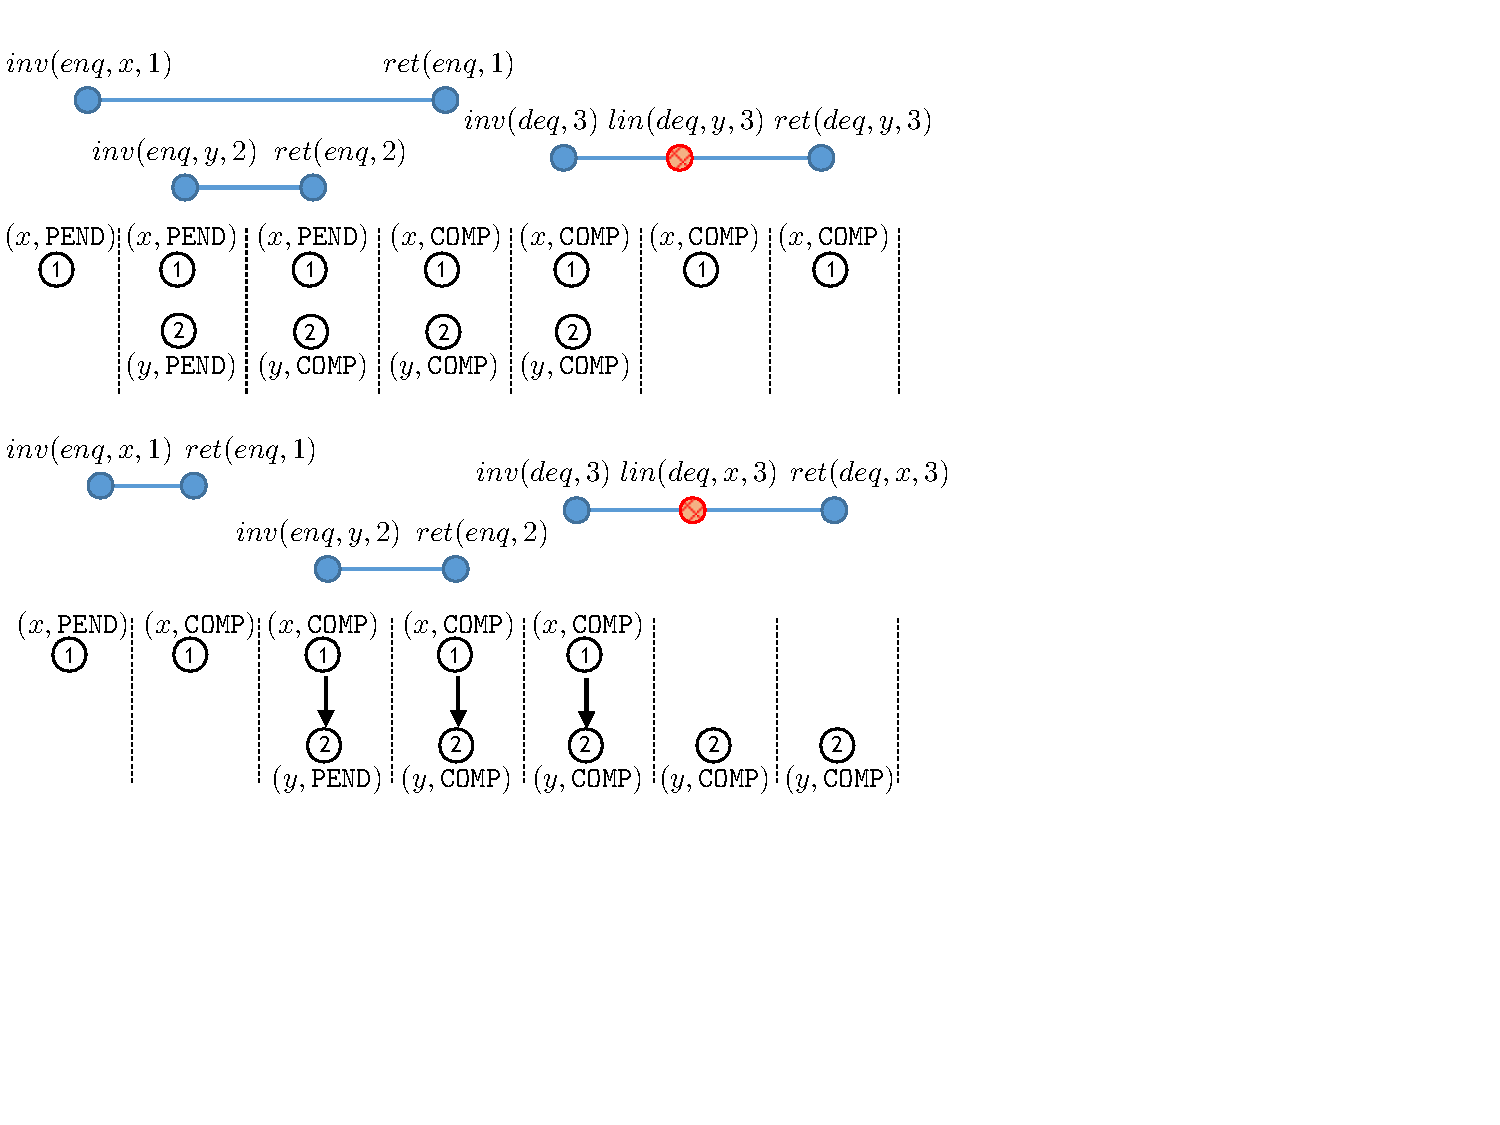
\includegraphics[width=7cm]{fig-queue12.pdf}
%
%\vspace{2mm}
%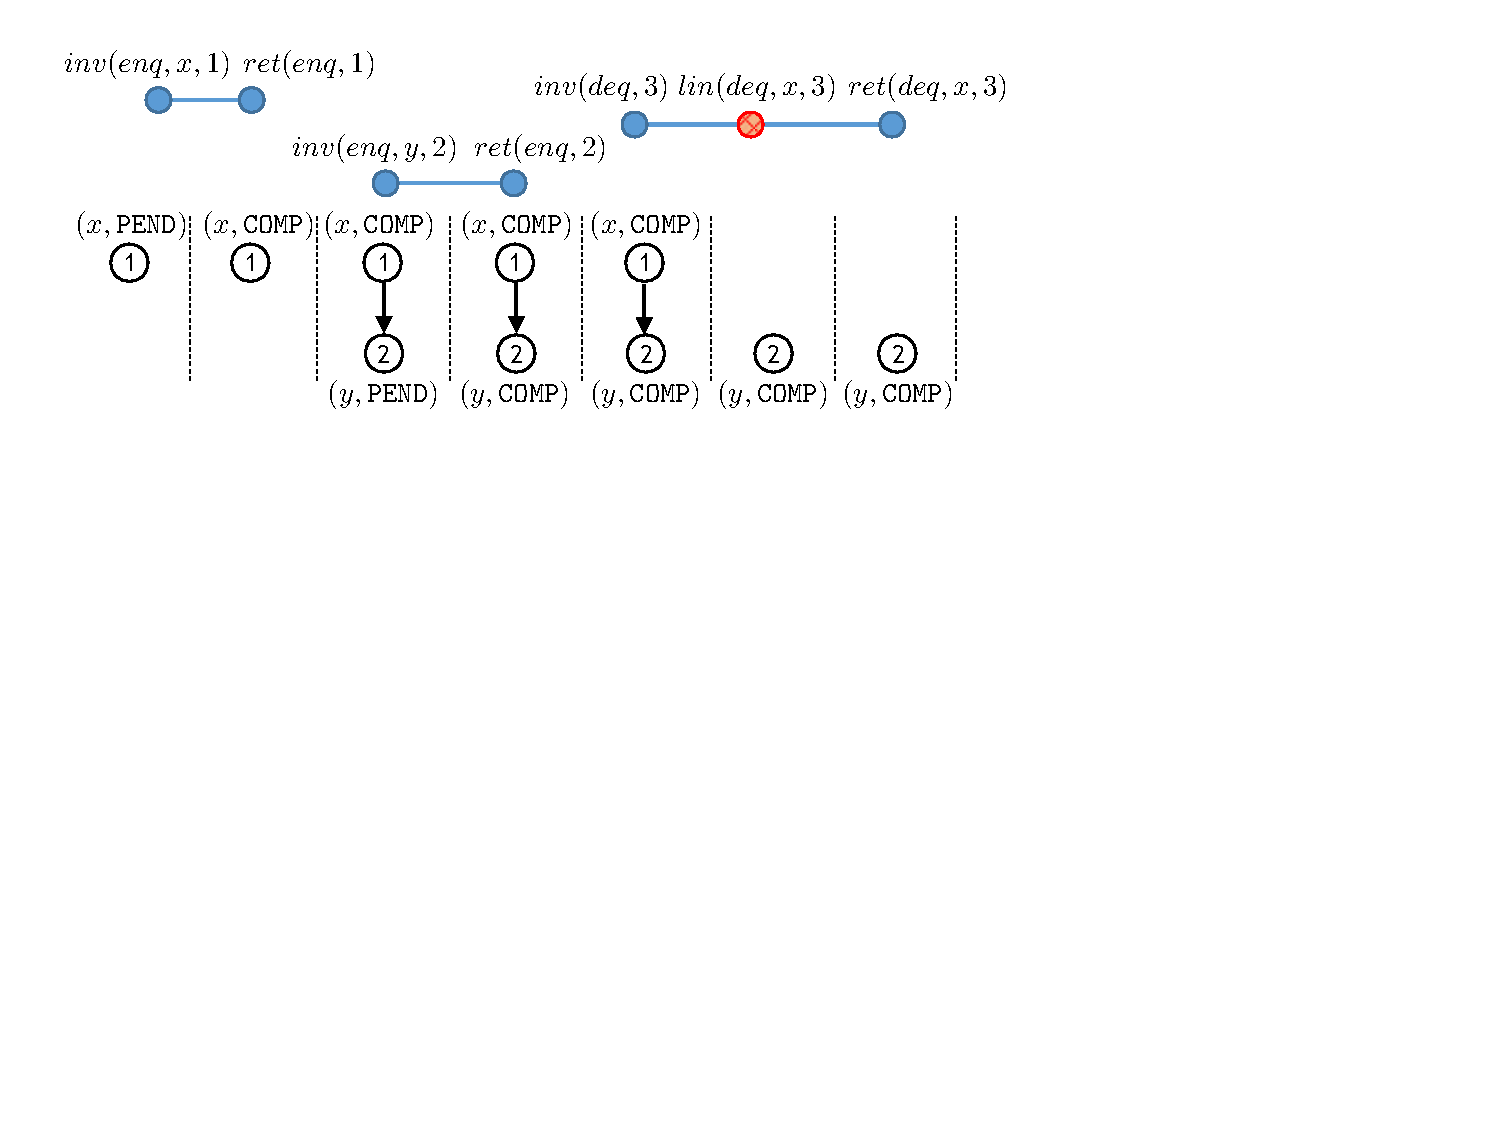
\includegraphics[width=7cm]{fig-queue2.pdf}
\vspace{-5mm}
\caption{Simulating queue histories with $AbsQ$.}
\label{fig:queueSim}
\vspace{-10mm}
\end{wrapfigure}
Figure 2 pictures two executions of $AbsQ$ for two extended histories (that include dequeue linearization points). The state of $AbsQ$ after each action is pictured as a graph below the action. The nodes of this graph represent enqueue operations and the edges happens-before constraints. Each node is labeled by a value (the input of the enqueue) and a flag {\tt PEND} or {\tt COMP} showing whether the operation is pending or completed. For instance, in the case of the first history, the dequeue linearization point $lin(deq,y,3)$ is enabled because the current happens-before contains a \emph{minimal} enqueue operation with input $y$. Note that a linearization point $lin(deq,x,3)$ is also enabled at this state.

Formally, the states of $AbsQ$ are tuples $\tup{O,<,\ell,rv,cp}$ where $O\subseteq \<Ops>$ represents a set of operation identifiers (of previously invoked enqueue operations), $<\subseteq O\times O$ is a strict partial order, $\ell: O -> \<Vals>\times\{\tt{PEND,\tt{COMP}}\}$ labels every identifier with a value and a flag that records whether the operation is pending or completed (this flag is used to track the happens-before order), $rv:\<Ops> ~> \<Vals>$ records the return value of a pending dequeue fixed at its linearization point ($~>$ denotes a partial function), and $cp:\<Ops> ~> \<Nats>$ records the control point of every pending (enqueue or dequeue) operation.
The initial state has all these components set to $\emptyset$ and the transition relation $->$ is defined in Figure~\ref{fig:transitions:AbsQ}. The alphabet of $AbsQ$ contains call/return actions and dequeue linearization points. The latter are denoted by $lin(deq,d,k)$ where $d\in \<Vals>$ and $k\in\<Ops>$. $Lin(deq)$ is the set of all such actions.

Concerning enqueue operations, the rule {\sc call-enq} orders the invoked operation after all the completed enqueue operations stored in the current state, and the rules {\sc ret-enq1}/{\sc ret-enq2} flip the corresponding flag from {\tt PEND} to {\tt COMP} provided that the operation is still present in the current state. For dequeue operations, {\sc call-deq} has no effect other than incrementing the control point and {\sc ret-deq} checks whether the return value is the same as the one fixed at the linearization point. The linearization point rule {\sc lin-deq1} corresponds to the case of a non-empty queue, showing that $lin(deq,d,k)$ is enabled only if the value $d$ has been added by an enqueue which is minimal in the current happens-before order. When it is enabled, it removes the enqueue adding $d$ from the state. The linearization point rule {\sc lin-deq2} corresponds to the case of dequeue operations linearized with an {\tt EMPTY} return value.

\begin{figure} [t]
{\scriptsize
  \centering
  \begin{mathpar}
    \inferrule[call-enq]{
      k\not\in dom(cp) \\ 
      d\neq {\tt EMPTY}
    }{
      O,<,\ell,rv,cp
      \xrightarrow{inv(enq,d,k)}
      %O\cup\{k\},<\cup \{(k',k): \ell_2(k')={\tt COMP}\},\ell[k\mapsto (d,{\tt PEND})],rv,cp[k\mapsto 1]
      O\cup\{k\},<\cup\ {\tt COMP}(O)\times\{k\},\ell[k\mapsto (d,{\tt PEND})],rv,cp[k\mapsto 1]
    }\hspace{5mm}

    \inferrule[call-deq]{
      k\not\in dom(cp) \\ 
    }{
      O,<,\ell,rv,cp
      \xrightarrow{inv(deq,k)}
      O,<,\ell,rv,cp[k\mapsto 1]
    }\hspace{5mm}
    \inferrule[ret-deq]{
       cp(k) = 2 \\
       rv(k)=d  
    }{
      O,<,\ell,rv,cp
      \xrightarrow{ret(deq,d,k)}
      O,<,\ell,rv,cp[k\mapsto 3]
    }\hspace{5mm}

    \inferrule[ret-enq1]{
      cp(k) = 1 \\
      k \in O \\
      \ell(k) = (d,{\tt PEND}) 
    }{
      O,<,\ell,rv,cp
      \xrightarrow{ret(enq,k)}
      O,<,\ell[k\mapsto (d,{\tt COMP})],rv,cp[k\mapsto 2]
    }\hspace{5mm}
    \inferrule[ret-enq2]{
      cp(k) = 1 \\
      k \not\in O 
    }{
      O,<,\ell,rv,cp
      \xrightarrow{ret(enq,k)}
      O,<,\ell,rv,cp[k\mapsto 2]
    }\hspace{5mm}

    \inferrule[lin-deq1]{
       cp(k) = 1 \\
       d\neq{\tt EMPTY} \\
       k'\in min(O) \land \ell_1(k')=d
    }{
      O,<,\ell,rv,cp
      \xrightarrow{lin(deq,d,k)}
      O\setminus \{k'\},<\uparrow k',\ell,rv[k\mapsto d],cp[k\mapsto 2]
    }\hspace{5mm}

    \inferrule[lin-deq2]{
       cp(k) = 1 \\
       \forall o\in O. \ell_2(o)={\tt EMPTY}
    }{
      O,<,\ell,rv,cp
      \xrightarrow{lin(deq,{\tt EMPTY},k)}
      O,<,\ell,rv[k\mapsto {\tt EMPTY}],cp[k\mapsto 2]
    }\hspace{5mm}

    
      \end{mathpar}
  }
 \vspace{-5mm}
  \caption{The transition relation of $AbsQ$. We use the following notations: $\ell_i(k)$ denotes the projection of $\ell(k)$ over the $i$-th component, for each $i\in\{1,2\}$, ${\tt COMP}(O)=\{k\in O: \ell_2(k)={\tt COMP}\}$, $\mathit{f}[x\mapsto y]$ is the function $g$ such that $g(z)=f(z)$ for all $z\neq x$ in the domain of $f$, and $g(x)=y$, $min(O)$ is the set of elements of $O$ which are minimal in the order relation $<$, and $<\uparrow k$ denotes the relation $<$ where all the pairs containing $k$ have been removed.
  %\textcolor{red}{Call-Enq must have $d!= \texttt{EMPTY}$ as a premise. Also lin deq returning empty must be changed as before.}
  }
  \label{fig:transitions:AbsQ}
\vspace{-6mm}
\end{figure}

Both methods have a fixed linearization point when the update of the shared sequence happens. Let $AbsQ_0$ denote this implementation~\footnote{For $\<Methods>=\{enq,deq\}$, the alphabet of $AbsQ_0$ is $C\cup R\cup Lin$.} (formally defined in Appendix~\ref{app:absImplQueue}).
The following result states that the library $AbsQ$ has exactly the same set of histories as the standard abstract library $AbsQ_0$ (see Appendix~\ref{app:absImplQueue} for a proof).

\begin{theorem}\label{th:absImplQueue}
$AbsQ$ is a refinement of $AbsQ_0$ and vice-versa.
\end{theorem}

A trace of a queue implementation is called \emph{$Lin(deq)$-complete} when every completed dequeue has a linearization point, i.e., TODO. A queue implementation $L$ over alphabet $\Sigma$ is called \emph{with fixed dequeue linearization points} if{f} $C\cup R\cup Lin(deq)\subseteq \Sigma$ 
and every trace $@t\in Tr(L)$ is $Lin(deq)$-complete.

TODO NEEDS DATA INDEPENDENCE FOR THE LINEARIZATION POINT TRANSITIONS TO BE DETERMINISTIC

The following result shows that $C\cup R\cup Lin(deq)$-forward simulations are a sound and complete proof method for showing the correctness of a queue implementation with fixed dequeue linearization points (up to the correctness of the linearization points). It is obtained from Theorem~\ref{th:absImplQueue} and Theorem~\ref{th:forSim} using the fact that the alphabet of $AbsQ$ is exactly $C\cup R\cup Lin(deq)$ and $AbsQ$ is deterministic.

\begin{corollary}
A queue implementation $L$ with fixed dequeue linearization points is a $C\cup R\cup Lin(deq)$-refinement of $AbsQ_0$ if{f} there exists a $C\cup R\cup Lin(deq)$-forward simulation from $L$ to $AbsQ$.
\end{corollary}

\subsection{A Correctness Proof For Herlihy\&Wing Queue}\label{ssec:HerlihyWing}

We describe a forward simulation $\mathit{fs}$ from $\mathit{HWQ}$ to $AbsQ$. Essentially, an $AbsQ$ state associated by $\mathit{fs}$ to a $\mathit{HWQ}$ state consists of all the  enqueue operations for which the input is still present in the array {\tt items} and all the pending enqueue operations that have at most reserved an array position, ordered by a relation $<$ satisfying the following: 
\begin{itemize}
	\item[(a)] pending enqueues are maximal, i.e., for every two enqueues $k$ and $k'$ such that $k'$ is pending, we have that $k'\not< k$,
	\item[(b)] $<$ is consistent with the order in which positions of {\tt items} have been reserved, i.e., for every two enqueues $k$ and $k'$ such that ${\tt i}(k) < {\tt i}(k')$, we have that $k' \not< k$,
	\item[(c)] an enqueue which has reserved an array position $i$ %and executed only the first statement 
	can't be ordered before another enqueue that has reserved a position $j \geq i$ when the position $i$ has been ``observed'' by a non-linearized dequeue that may ``observe'' $j$ in the current array traversal, i.e., for every two enqueues $k$ and $k'$, and a dequeue $k_d$, such that 
	
	\noindent
	{\small
	\begin{align}
	\hspace{-8mm}
	{\tt x}(k_d)={\tt null} \land {\tt i}(k') \leq {\tt range}(k_d) \land {\tt i}(k) \leq {\tt i}(k_d) \leq {\tt i}(k')
	 \land ({\tt i}(k) = {\tt i}(k_d) => k_d\atCP {\tt if}\text{-}{\tt inc}) \label{eq:inst}
	\end{align}}
	
	\noindent
	we have that $k \not< k'$. The predicate $k_d\atCP {\tt if}\text{-}{\tt inc}$ holds when the dequeue $k_d$ is at a control point after a {\tt swap} returning {\tt null} and before the increment of {\tt i}.
\end{itemize}

An enqueue is labeled by $(d,{\tt PEND})$ where $d$ is the input value if it's pending and by  $(d,{\tt COMP})$, otherwise. Also, for every dequeue operation $k$ such that ${\tt x}(k)=d\neq {\tt null}$, we have that $rv(k)=d$.

We show that $\mathit{fs}$ is indeed a $C\cup R\cup Lin(deq)$-forward simulation. Let $s$ and $t$ be states of $\mathit{HWQ}$ and $AbsQ$, respectively, such that $(s,t)\in\mathit{fs}$. 
We omit discussing the trivial case of transitions labeled by call and return actions (for the return a dequeue operation $k$, we use the equality between the local variable ${\tt x}(k)$ in $s$ and the component $rv(k)$ in $t$). \textcolor{red}{ I think it is good to mention again that call/return actions in HWQ correspond to the same call/return actions in AbsQ (without any other internal action). I also think that invoke enqueue operation is non-trivial. Preservation of the strict partial order and all of the above items a, b and c needs to be rechecked.}

We show that each internal step of an enqueue or dequeue, except the execution of {\tt swap} returning a non-null value in dequeue (which represents its linearization point), is simulated by an \emph{empty} sequence of $AbsQ$ transitions, i.e., for every state $s'$ obtained through one of these steps, if $(s,t)\in\mathit{fs}$, then $(s',t)\in\mathit{fs}$ for each $AbsQ$ state $t$. We focus on the following essential property, called \emph{monotonicity}: the set of possible orders $<$ associated by $\mathit{fs}$ to $s'$ doesn't exclude any order $<$ associated to $s$.
%Essentially, this boils down to showing that the constraints over $<$ in the definition of $\mathit{fs}$ are an invariant for these steps.

Concerning enqueues, let $s'$ be the state obtained from $s$ when a pending enqueue $k$ reserves an array position. This enqueue operation must be maximal in both $t$ and any state $t'$ related to $s'$ (because it is pending). Moreover, there is no dequeue that can ``observe'' this position before restarting the array traversal. Therefore, item (c) in the definition of $<$ doesn't constrain the order between $k$ and some other enqueue neither in $s$ nor in $s'$. Since this transition doesn't affect the constraints on the order between enqueue operations different from $k$ (their local variables remain unchanged), we have that monotonicity holds. This property is trivially satisfied by the second step of enqueue which doesn't affect {\tt i}.

To prove monotonicity in the case of dequeue internal steps different from its linearization point, it is important to track the non-trivial instantiations of item (c) in the definition of $<$ over the two states $s$ and $s'$., i.e., the triples $(k,k',k_d)$ for which (\ref{eq:inst}) holds. Instantiations that are enabled only in $s'$ may in principle lead to a violation of monotonicity (since they restrict the orders $<$ associated to $s'$). For the two steps that begin an array traversal, i.e., reading the index of the last used position and setting the iterator {\tt i} to $0$, there exist no  such new instantiations in $s'$ because the value of {\tt i} is either not set or $0$. % (it is trivial to notice that applying these steps doesn't disable such instantiations that were possible in $s$). 
%The same holds for the step incrementing the iterator {\tt i}. 
%
%The execution of {\tt swap} returning {\tt null} may introduce one new non-trivial instantiation $(k,k',k_d)$ of item (c).
%We write ${\tt i}_s(k)$ to refer to the value of the variable {\tt i} of operation $k$ in state $s$. Assume that indeed, there exist two enqueue operations $k$ and $k'$ such that ${\tt i}_{s'}(k) < {\tt i}_{s'}(k_d) \leq {\tt i}_{s'}(k')$, ${\tt x}_{s'}(k_d)={\tt null}$, ${\tt i}_{s'}(k') \leq {\tt range}_{s'}(k_d)$ TODO SWAP. Since {\tt swap} returnes {\tt null}, the position ${\tt i}_{s'}(k_d)$
%
%
% and ${\tt i}_{s}(k) = {\tt i}_{s'}(k_d)$. The latter constraint guarantees that this instantiation is not enabled in state $s$. The increment of {\tt i} being enabled, implies that 
%
The same is true for the increment of the iterator {\tt i} in a dequeue $k_d$ since the predicate $k_d\atCP {\tt if}\text{-}{\tt inc}$ holds in state $s$.
The execution of {\tt swap} returning {\tt null} in a dequeue $k_d$ enables new instantiations $(k,k',k_d)$ in $s'$, thus adding potentially new constraints $k\not< k'$. We show however that these instantiations are vacuous because $k$ must be a pending enqueue in $s$ and thus maximal in any order relation $<$ associated by $\mathit{fs}$ to $s$.
Let $k$ and $k'$ be two enqueue operations such that together with the dequeue $k_d$ they satisfy the property (\ref{eq:inst}) in $s'$ but not in $s$. 
We write ${\tt i}_s(k)$ to refer to the value of the variable {\tt i} of operation $k$ in state $s$. 
This implies that ${\tt i}_{s'}(k) = {\tt i}_{s'}(k_d) \leq {\tt i}_{s'}(k')$ and ${\tt items}[{\tt i}_{s'}(k_d)]={\tt null}$. The latter implies that the enqueue $k$ didn't executed
the second statement and it is pending (because the position it reserved is still {\tt null}). Finally, checking whether the value returned by {\tt swap} is {\tt null} doesn't modify any of the variables in property  (\ref{eq:inst}) and also, it doesn't change the valuation of the predicate $\atCP {\tt if}\text{-}{\tt inc}$.

TODO LINEARIZATION POINT
